\chapter{Distance control}
In this chapter, the focus will be on modeling and the control of the distance between two satellites using the drag force as the control input of the system. First, it is considered that the orientation of the satellite is instantaneous and therefore, the drag force can be modified instantaneously. The Earth and the satellite are assumed to be a point mass to simplify the system.
\section{Modelling}
The Satellite is mainly subjected to three forces: the gravity, the drag force and the sun radiation. Thus, the second law of Newton gives:
\begin{flalign}
 \sum {F} = m_{sat} \ a = {F_g} + {F_D} + {F_{rad}}
	\label{eq:ecc}
\end{flalign}
with the gravity modeled by:
\begin{flalign}
{F_g} = -G\frac{m_{earth} \cdot m_{sat}}{||{p}||^3} {p}
	\label{eq:eccc}
\end{flalign}
where ${p}$ is the vector position of the satellite (vector from the earth center to the mass center of the satellite in the inertial frame) and the expresion for ${F_D}$ and ${F_{rad}}$ are explained in the next section.
\section{Disturbance Models}
\subsection{Aerodynamic Drag Force}
The satellite is subjected to an aerodynamic drag force due to the atmosphere. The collisions with the air cause a force in the opposite direction of the velocity of the satellite. The force was modeled by Lord Rayleigh.\cite{FSA}
\begin{flalign}
{F_D} = -\frac{1}{2} \rho \cdot C_D \cdot A_{\perp} ||{v}|| \ {v}
	\label{eq:ec1c}
\end{flalign}
where $\rho$ is the density of the air, $C_D$ is the drag coefficient, $A_{\perp}$ is the area that is perpendicular of the velocity of the satellite ${v}$. 

The drag coefficient $C_D$ and the perpendicular area $A_{\perp}$ depend on the orientation of the satellite. Therefore, this force can be used as an input for the control of the position and the velocity of the satellite.

The density of the air depends on the altitude of the satellite, of the air temperature but we considered to be constant in our case to simplify the model.\textbf{ $\rho$ is chosen to be equal to $1.454 \cdot 10^{-13} Kg/{m^3}$ based on the  empirical model of the Committee on Space Research (COSPAR) International Reference Atmosphere \cite{SADC}.}

The drag coefficient as said before is orientation dependent. The maximum value of $C_D$ is equal to 1.05 for a non tilted cubed as shown on the figure \figref{fig:drag} and equal to 0.80 for an angled cubed \cite{wik}. \textbf{In our modelization, we will assume that the drag coefficient is constant and equal to 1(not sure which value take) in order to simplified the equation. }
\begin{table}[H]
	\begin{minipage}[b]{0.49\linewidth}
		\centering
		\begin{figure}[H]
			\centering
			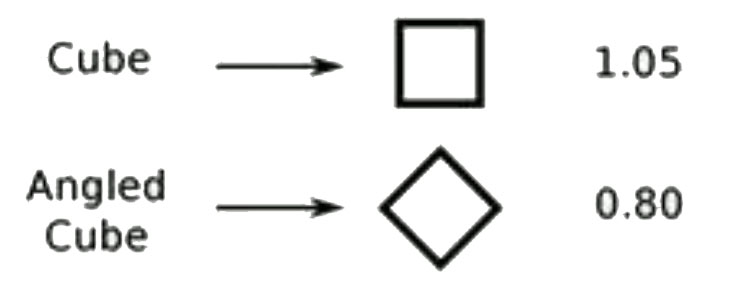
\includegraphics[width=0.8\linewidth]{figures/drag_coef}
			\caption{description needed}
			\label{fig:drag}
		\end{figure}
	\end{minipage}\hfill
	\begin{minipage}[b]{0.49\linewidth}
		\centering
		\begin{figure}[H]
			\centering
			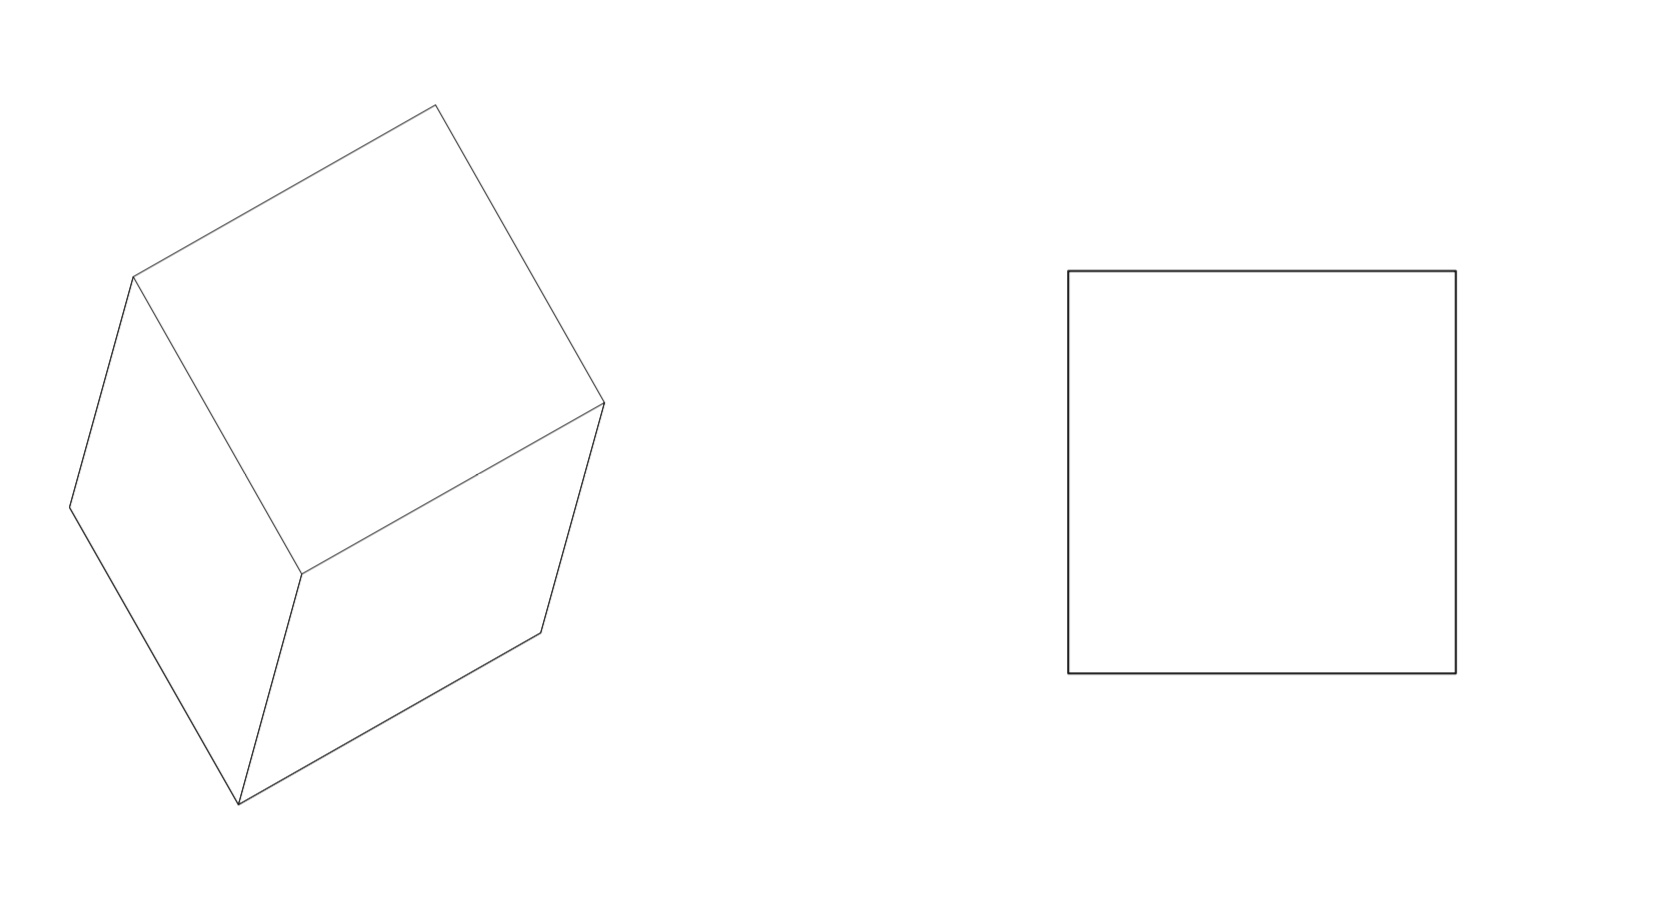
\includegraphics[width=1\linewidth]{figures/a_prep}
			\caption{description needed}
			\label{fig:cub}
		\end{figure}
	\end{minipage}
\end{table}
Therefore, the control parameter is the perpendicular area $A_{\perp}$. The maximum and minimum value of $A_{\perp}$ are represented in \figref{fig:cub}. Thus, the minimum value is the surface of a square of 10cm of dimension ($A_{\perp} = 100cm^2$) and the maximum value is the surface of an hexagone of 10cm of dimension ($A_{\perp} = \frac{3\sqrt{3}}{2} 100cm^2$).
Thus, the drag force can be expressed as the following. 
\begin{flalign}
{F_D} = -u ||{v}|| {v}
\label{eq:teor}
\end{flalign}
where $u$ is the control input and it can take value between $7.27 \cdot 10^{-16}$ and $1.888 \cdot 10^{-15}$
\subsection{Solar radiation}
Tfhe surface of the CubeSat will absorb or reflect the solar radiation, nevertheless, these two situations will alter the CubeSat, which will produce a torque about the satellite center of mass (CoM). \cite{SADC}

The torque around CoM is given by:
\begin{flalign}
N_{rad} = F_{rad} \times R_{CoM}
\label{eq:tor}
\end{flalign}
where $F_{rad}$  is the solar radiation  and $R_{CoM}$ is the vector from the centre of mass to the geometric centre of radiation

The solar radiation $F_{rad}$ can be expressed as:
\begin{flalign}
F_{rad} = C_{a} P A
\label{eq:Pres}
\end{flalign}
where $C_{a}$ is the surface’s reflectance: 0 for a perfect absorber, 1 for a perfect reflector,   while $P$ is the solar flux and  $A$ is the radiated area

The solar flux can be computed as follows:
\begin{flalign}
P = \dfrac{F_s}{c}
\label{eq:flux}
\end{flalign}
where $F_s$ is the mean solar energy and it is equal with 1358 $W/m^2$ and $c$ is the speed of light
\subsection{$J_2$ gravity perturbation}
A satellite orbiting the Earth encounter multiple perturbing forces. Some of these forces are the atmospheric drag, the gravity gradient, and the solar radiation. The influence of these forces upon the satellite is deemed to be negligible, but one perturbation produced by the oblateness of the Earth is taken into account because will provoke a change in the orientation of the orbit.

The force which the Earth is exerting upon a object outside its sphere is a conservative force and it can be written as follows:
\begin{flalign}
	U(r) = -\frac{\mu}{r}
	\label{eq:Pr}
\end{flalign}
Because the Earth is not a perfect sphere and also its mass distribution is not homogeneous, \eqref{eq:Pr} is rewritten by adding the spherical harmonic expansion to correct the gravitational potential for the Earth:
\begin{flalign}
		U(r) = -\frac{\mu}{r}+ B(r, \phi , \lambda)
	\label{eq:Pr1}
\end{flalign}
where $B(r, \phi, \lambda)$ is the spherical harmonic expansion used to correct the gravitational potential for the Earth's nonsymmetric mass distribution seen in \figref{fig:j2}
\begin{figure}[H]
	\centering
	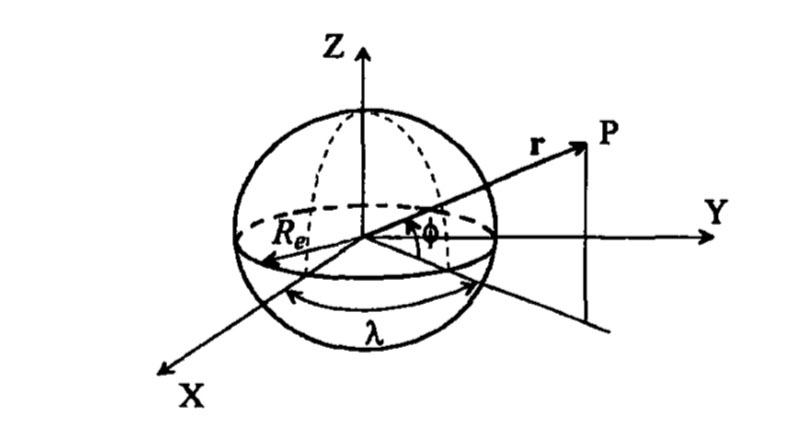
\includegraphics[width=0.6\linewidth]{figures/j2}
	\caption{Coordinates for deriving the external gravitational potential of the Earth }
	\label{fig:j2}
\end{figure} 
In order to solve the problem regarding the oblatness, the gravitational potential of the Earth is extended into series of spherical harmonics: [ref]
\begin{flalign}
	 B(r, \phi , \lambda) = \frac{\mu}{r} \left\{ \sum_{n=2}^{\infty} \left [ \left (\frac{R_e}{r} \right)^{n} J_n P_n sin(\phi)| +\sum_{m=1}^{n} \left (\frac{R_e}{r}\right)^{n} (C_{nm} cos(m\lambda) + S_{nm} sin(m\lambda)) P_{nm} sin(\phi)  \right] \right\}
	\label{eq:phi2}
\end{flalign}
where $r, \phi , \lambda$ are spherical coordinates and the parameteres from the function are defined as follows: $r$ is the geocentric distance of point $P$, $\phi$ is the geocentric latitude, $\lambda$ is the geographical longitude, $R_e$ is the mean equatorial radius of the Earth, $cos(m\lambda)$ and $sin(m\lambda)$ are harmonics in $\lambda$, $J_{nm}$ are the zonal harmonic coefficients, $J_n$ zonal harmonic coefficients of order 0, $P_{nm} $ associated Legendre polynomial of degree $n$ and order $m$, $P_n$ is Legendre polynomial degree $n$ and order 0, $C_{nm}$ is tesseral harmonic coefficients for $n \neq m$, $S_{nm}$ is sectoral harmonic coefficients for $n =m$

The expression for gravitational potential of the Earth can be approximate as:
\begin{flalign}
   U \approx -\frac{\mu}{r} \left[1 - \sum_{n=2}^{\infty} \left(\frac{R_e}{r}\right)^{n} J_n P_n sin(\phi)  \right ] = \frac{\mu}{r} [U_0 + U_{J_2} + U_{J_3} + ...]
	\label{eq:Pr341}
\end{flalign}
where $U_0$ = -1 and $U_{J_2}$ = $\left(\frac{R_e}{r}\right)^{2} J_2 \frac{1}{2} (3 sin^2 \phi -1) $

The gravitational forces acting on the satellite are obtained from the relation:
\begin{flalign}
	F = -m \nabla U
	\label{eq:Pr3431}
\end{flalign}
and is obtaining the following:
\begin{flalign}
	F_x = -\frac{\partial U}{\partial x} = \mu \left[ -\frac{x}{r^3} + A_{J_2} \left(15 \frac{xz^2}{r^7} - 3\frac{x}{r^5}   \right ) \right ]       \\
		F_y = -\frac{\partial U}{\partial y} = \mu \left[ -\frac{y}{r^3} + A_{J_2} \left(15 \frac{yz^2}{r^7} - 3\frac{y}{r^5}   \right ) \right ]       \\
			F_z = - \frac{\partial U}{\partial z} =  \mu \left[ -\frac{z}{r^3} + A_{J_2} \left(15 \frac{z^3}{r^7} - 3\frac{z}{r^5}   \right )  \right]       
	\label{eq:Pr34331}
\end{flalign}
where $A_{J_2}  = \frac{1}{2} J_2 R_e^2$ and and$R_e$ is the mean radius ofthe earth at the equator
	
\section{State Space Representation}
The state of the system is the vector position and the vector velocity in the inertial frame:
\begin{flalign}
{x} = \left[ \begin{array}{c} {p} \\ {v} \end{array} \right]
	\label{eq:Pr3341}
\end{flalign}
The equation of (I don't remember the name of the equation xdot = f(x,u) + u) is given by:
\begin{flalign}
\dot{x} &= \left[ \begin{array}{c} \dot{p} \\ \dot{v} \end{array} \right] = \left[ \begin{array}{c} {v} \\ {a} \end{array} \right] \\
 &= \left[ \begin{array}{c} {v} \\ \frac{1}{m_{sat}}(-G\frac{m_{earth} \cdot m_{sat}}{||{p}||^3} {p}) - u ||{v}|| {v} + F_{rad} \end{array} \right] \\
 &= {f(x)} + u \cdot {g(x)} + {\delta(x,t)}
\end{flalign}
with 
\[
{f(x)} = \left[ \begin{array}{c} {v} \\ -G\cdot m_{earth} \frac{p}{||{p}||^3} \end{array} \right], \ {g(x)} = \left[ \begin{array}{c} {0} \\ - \frac{1}{m_{sat}}||{v}||{v} \end{array} \right]
\]
and ${\delta(x,t)}$ reprensent the influence all the disturbances.
\section{Relative dynamics}
In order to analyse the distance between two satellites, the relative dynamics are analyzed. Furthermore, to simplify the system, satellites will be assumed to stay in the same plane. This assumption has also to be made due to the limitation of the direction of the input control (the drag force). \\
To compute the equations of the motion of one satellite compared to another, a new frame is used. The frame is illustrated in the figure \figref{fig:rel_dyn}, where the origin is the first satellite and the axis ${\hat{x}}$ is defined by ${\hat{x}} = \frac{{R}}{R}$ where ${R}$ is the vector from the center of the Earth to the first satellite, the axis ${\hat{y}}$ is perpendicular to ${\hat{x}}$ and in the plane of motion of the satellites and ${\hat{z}}$ is defined by the right-hand law (${\hat{z}} = {\hat{x}} \times {\hat{y}}$). \\
\begin{figure}[H]
	\centering
	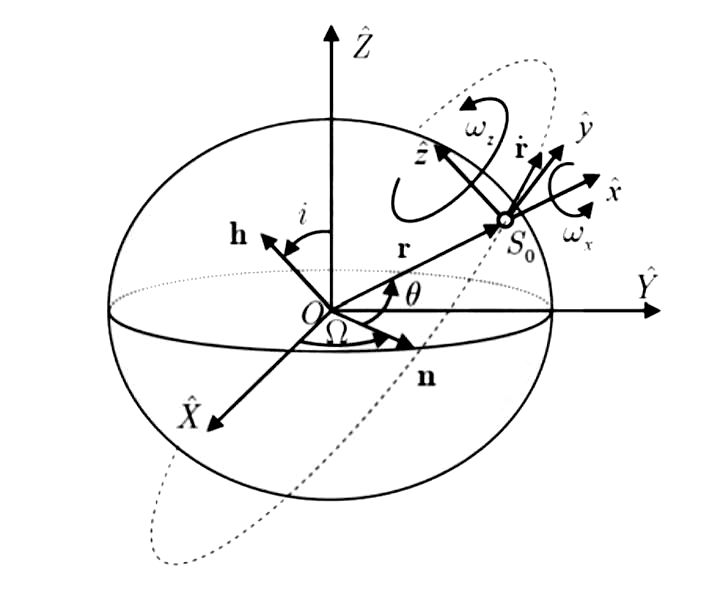
\includegraphics[width=0.6\linewidth]{figures/relativeDynamics}
	\caption{Frame for the relative dynamics}
	\label{fig:rel_dyn}
\end{figure} 
Therefore, the vector position from the Earth to the fist satellite and the second satellite can be expressed in this frame:
\begin{flalign}
{p_1} &= R \cdot {\hat{x}} \\
{p_2} &= R \cdot {\hat{x}} + x \cdot {\hat{x}} + y \cdot {\hat{y}} 
\end{flalign}
The equations of relative motions are derived in \appref{chap:B}.
%
\subsubsection{Relative state space representation}
%
Since the equations of relative motion  that have been derived in \appref{chap:B} are not linear, an approximation of a linearization is made around the operating points, $x*$ and $y*$, by introducing the states with a new variable as $s = [x; \dot{x}; y; \dot{y}]$, more about this can be found in \appref{chap:C}.  
%
In order to derive the linear state space model the assumptions that the radius is constant and that the angular velocity, $w = \sqrt{\frac{\mu}{R^3}}$ is constant, lead in the assumption that $\dot{R} = 0$ and $\dot{w} = 0$. Furthermore, using the approximation $\dot{x}$, $y << y^{*}$ and $x, x^{*}$, $\frac{\dot{y}}{w} << R$, the \eqref{eq:statespaceassumption} has been derived. Finally assuming that $y* << R$ the linear system can be written in state space form  
%
 \begin{flalign*}
 	{\dot{x}(t)} ={A x(t) + Bu(t)}
 \end{flalign*}  
 \begin{flalign*}
	{y(t)} ={ C x(t) + D u(t)}
\end{flalign*} 
%
as
%
\begin{flalign*}
	{A}
	= 
	\begin{bmatrix}
		0& 1& 0 & 0 \\
		0& 0&0&2w  \\ 
		0&0&0&1 \\
		0&-2w & 0 &0
	\end{bmatrix} 
\end{flalign*}
\begin{flalign*}
	{B}
	= 
	\begin{bmatrix}
		0& \\
		0&  \\ 
		0& \\
		-Rw&
	\end{bmatrix} 
\end{flalign*}
%
$C=eye(4) $ and $D =0$.
%
With this assumptions and by using a control law $u= u_2 - u_1$ from the \eqref{eq:statespaceassumption} it can be seen that when $u_2 > u_1$ then $u>0$ and in this case $y$ should have a decreasing attitude as seen in the \figref{fig:theoryapprox}
%
\begin{figure}[H]
\centering
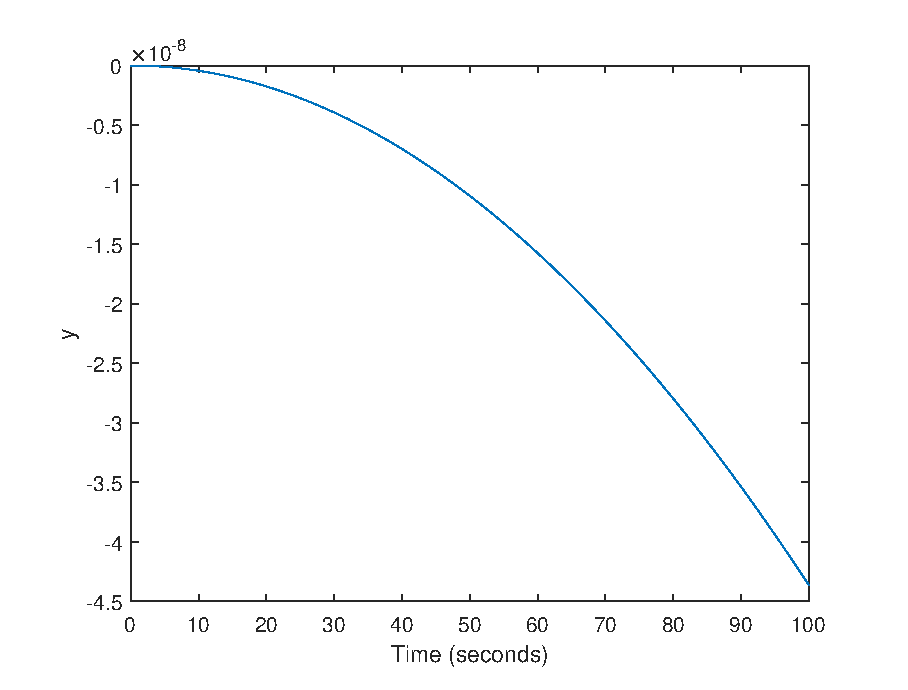
\includegraphics[width=0.6\linewidth]
{figures/theoryapprox.eps}
\caption{Theoretical decreasing attitude of y }
\label{fig:theoryapprox}
\end{figure}
% 
Taking into account all the above assumptions, this theoretical attitude of $y$ should be the same with the results from the actual model simulation, in order to proceed to the design of the controller. From the \figref{fig:practiceapprox} 
%  
\begin{figure}[H]
	\centering
	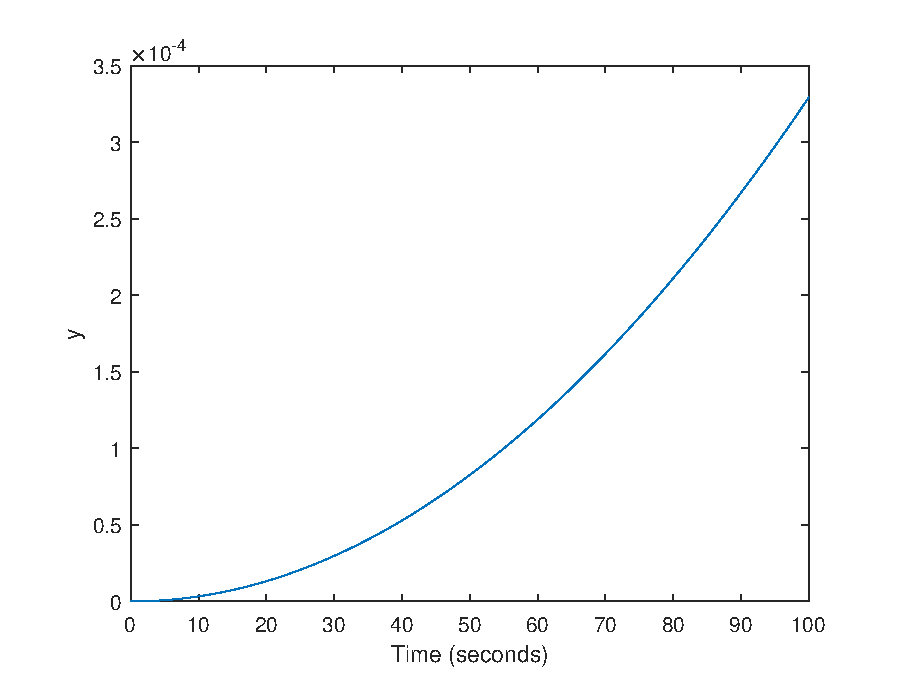
\includegraphics[width=0.6\linewidth]
	{figures/practiceapprox.eps}
	\caption{The practical attitude of y is increasing }
	\label{fig:practiceapprox}
\end{figure}
% 
it can be seen that the theoretical with the practical attitude of $y$  are not the same. This is due to the fact that as the drag force is becoming higher, the energy of the satellite is decreasing leading in increasing angular velocity with direction to the earth. Furthermore, when $u_2 > u_1$, then $w_2 > w_1$. This will lead to an increase in the angle $\theta$ between the satellites, and since $y = Rsin\theta$, $y$ will have increasing attitude. The above mentioned issues are shown in \figref{fig:inomega} which is the simulation for $w$ and in  \figref{fig:intheta} which is for $\theta$.    
%
\begin{figure}[H]
	\centering
	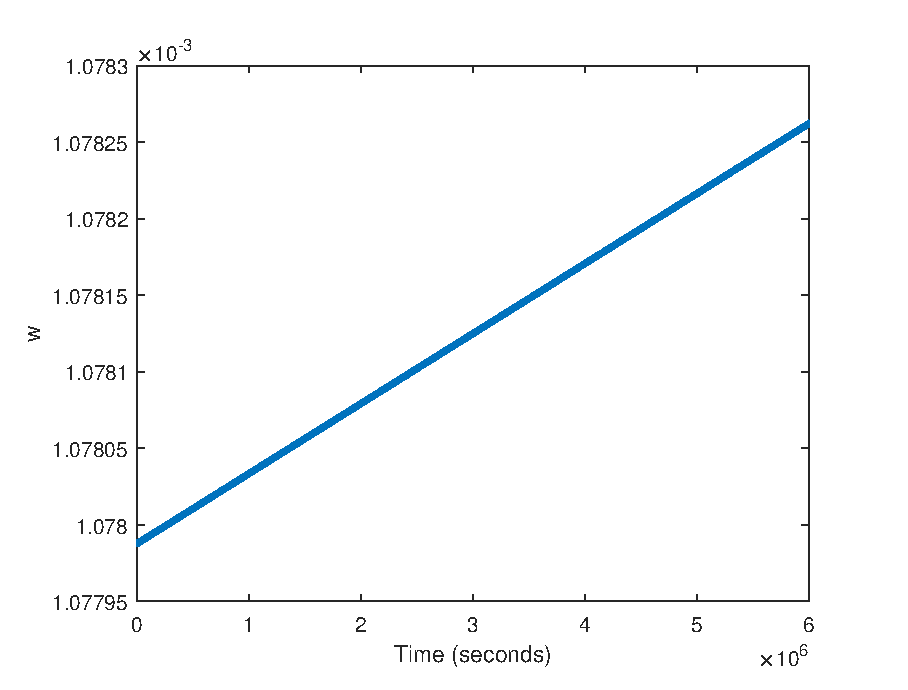
\includegraphics[width=0.6\linewidth]
	{figures/nonomega.eps}
	\caption{For $u_2 >u_1$, $w$ is increasing  }
	\label{fig:inomega}
\end{figure}
%
\begin{figure}[H]
	\centering
	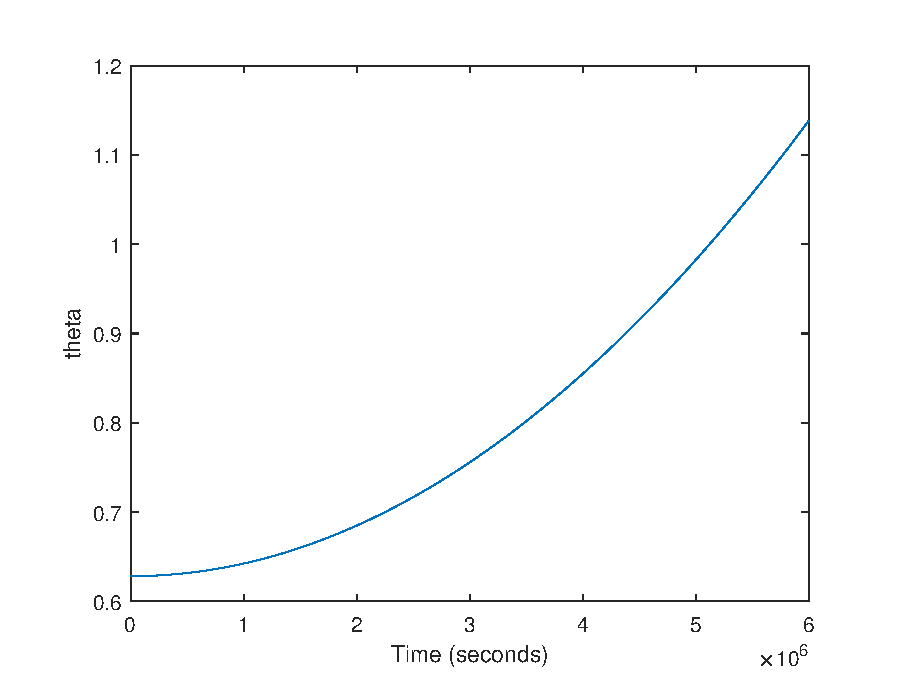
\includegraphics[width=0.6\linewidth]
	{figures/nontheta.eps}
	\caption{For $u_2 >u_1$, $\theta$ is increasing }
	\label{fig:intheta}
\end{figure}
%
 Since the approximations that have been made are not sufficient and there is not enough control authority, this set up has not deemed good enough for implementation. 
%
\section{Modelling based on the angular velocity}
As seen in the previous section, the angular velocity can not be assumed constant. Therefore a equation is needed to estimate it in function of the drag force. In the appendix D, the time derivative of the angular velocity can be approximated as a linear function of the drag force. 
\begin{flalign}
	\dot{\Delta \omega} = C u
\end{flalign}
with $C = \frac{3 \omega_0^2 R_0}{m}$. In order to check this equation and the coefficient, a simulation is performed using a constant drag force coefficient ($u = \frac{u_{min} + u_{max}}{2}$). The angular velocity as a function of time with constant drag force is shown in \figref{fig:testCoef}. \\
\begin{figure}[H]
	\centering
	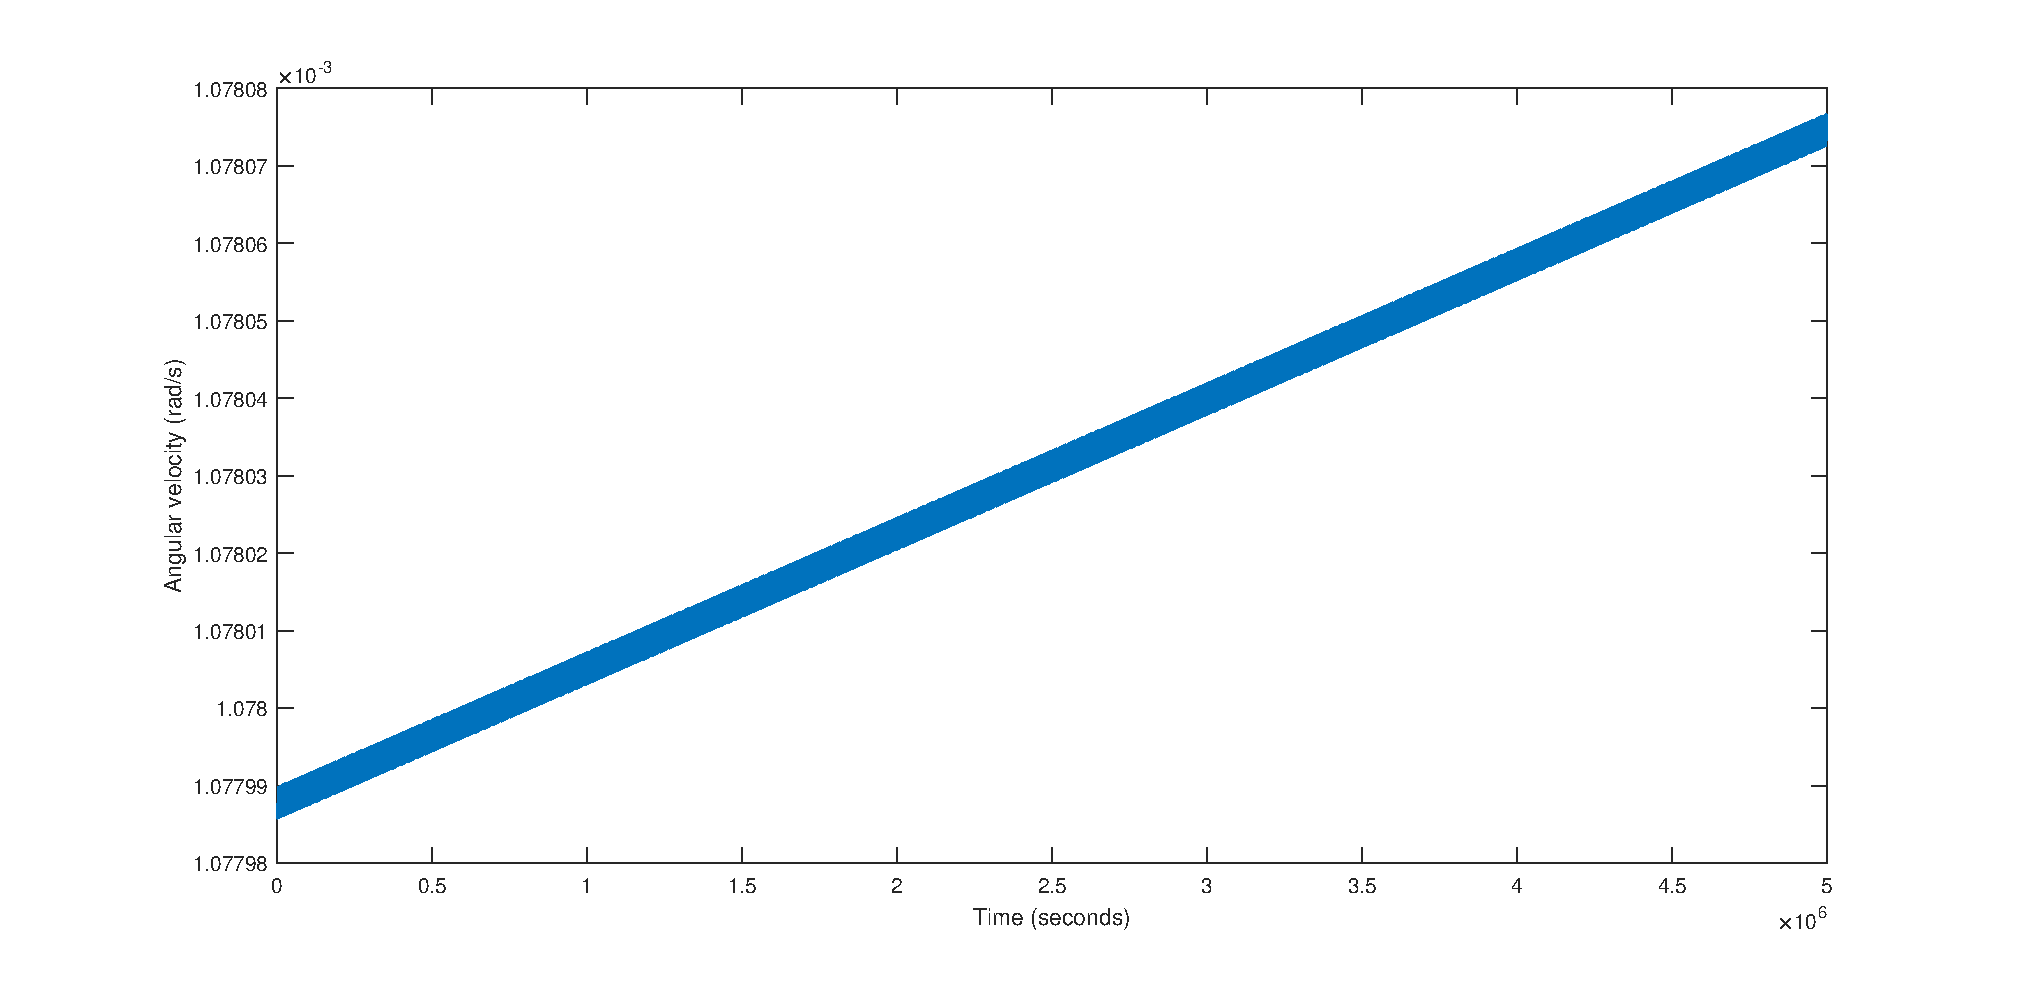
\includegraphics[width=0.9\linewidth]
	{figures/test_coef.eps}
	\caption{Angular velocity in function of time}
	\label{fig:testCoef}
\end{figure} 
The coefficient found in the simulation is almost the same than in the theory and oscillations can be observed with a frequency equals to $f \approx \frac{2\pi}{\omega_0}$. This is due to the fact that the orbit is not exactly a circle but a ellipse. Thus, The angular velocity changes a little during a turn around the Earth. In order to limit the influence of these variations on the controller, A low pass filter will be added to reduce the amplitude of these oscillations. \\
A state space representation can be derived:
\begin{flalign}
	{s}
	= 
	\begin{bmatrix}
		\theta - \theta_{ref} \\
		\dot{\theta}
	\end{bmatrix} 
\end{flalign}
\begin{flalign}
	&{\dot{s}(t)} ={A s(t) + Bu(t)}
	\label{eq:statespacecomplex}
\end{flalign}  
where
\begin{flalign}
	{A}
	= 
	\begin{bmatrix}
		0& 1& \\
		0& 0&
	\end{bmatrix} 
\end{flalign}
\begin{flalign}
	{B}
	= 
	\begin{bmatrix}
		0& \\
		\frac{3 \omega_0^2 R_0}{m}
	\end{bmatrix} 
\end{flalign}
and $u = u_2 - u_1$ and $\theta$ is the angle between two satellites.
\section{Distance control design}\label{46}
A controller is designed to control the angle between two satellites. Due to the fact that the state representation is linear, Linear Quadratic Regulator(LQR) is choosen as control method with weights as  
\begin{flalign}
	{Q}
	= 
	\begin{bmatrix}
		(\frac{pi}{3})^{-2}& 0& \\
		0& 0&
	\end{bmatrix} 
\end{flalign}
\begin{flalign}
	{R}
	= 
	\begin{bmatrix}
		u_{max}^{-2}
	\end{bmatrix} 
\end{flalign}
 The vector of gain K is obtained using the command \textit{lqr(A,B,C,D,[])} in Matlab. The control input signal can be computed ($u = u_2 - u_1$) and therefore if u is bigger than zero, $u_1$ will be equal to $u_{min}$ and $u_2$ will be equal to $u + u_{min}$. If u is smaller than zero, it will be the opposite.
\subsubsection{Frequency Analysis}
The loop transfer function can be computed L(s) = P(s)C(s)LPF(s) where P(s) is the transfer function of the state representation system, C(s) = $K_1$ + $K_2$s is the transfer function of the controller and LPF(s) is the transfer function of the low pass filter.
The bode diagram of L(s) is represented in the \figref{fig:Bode_L}. \\
\begin{figure}[H]
	\centering
	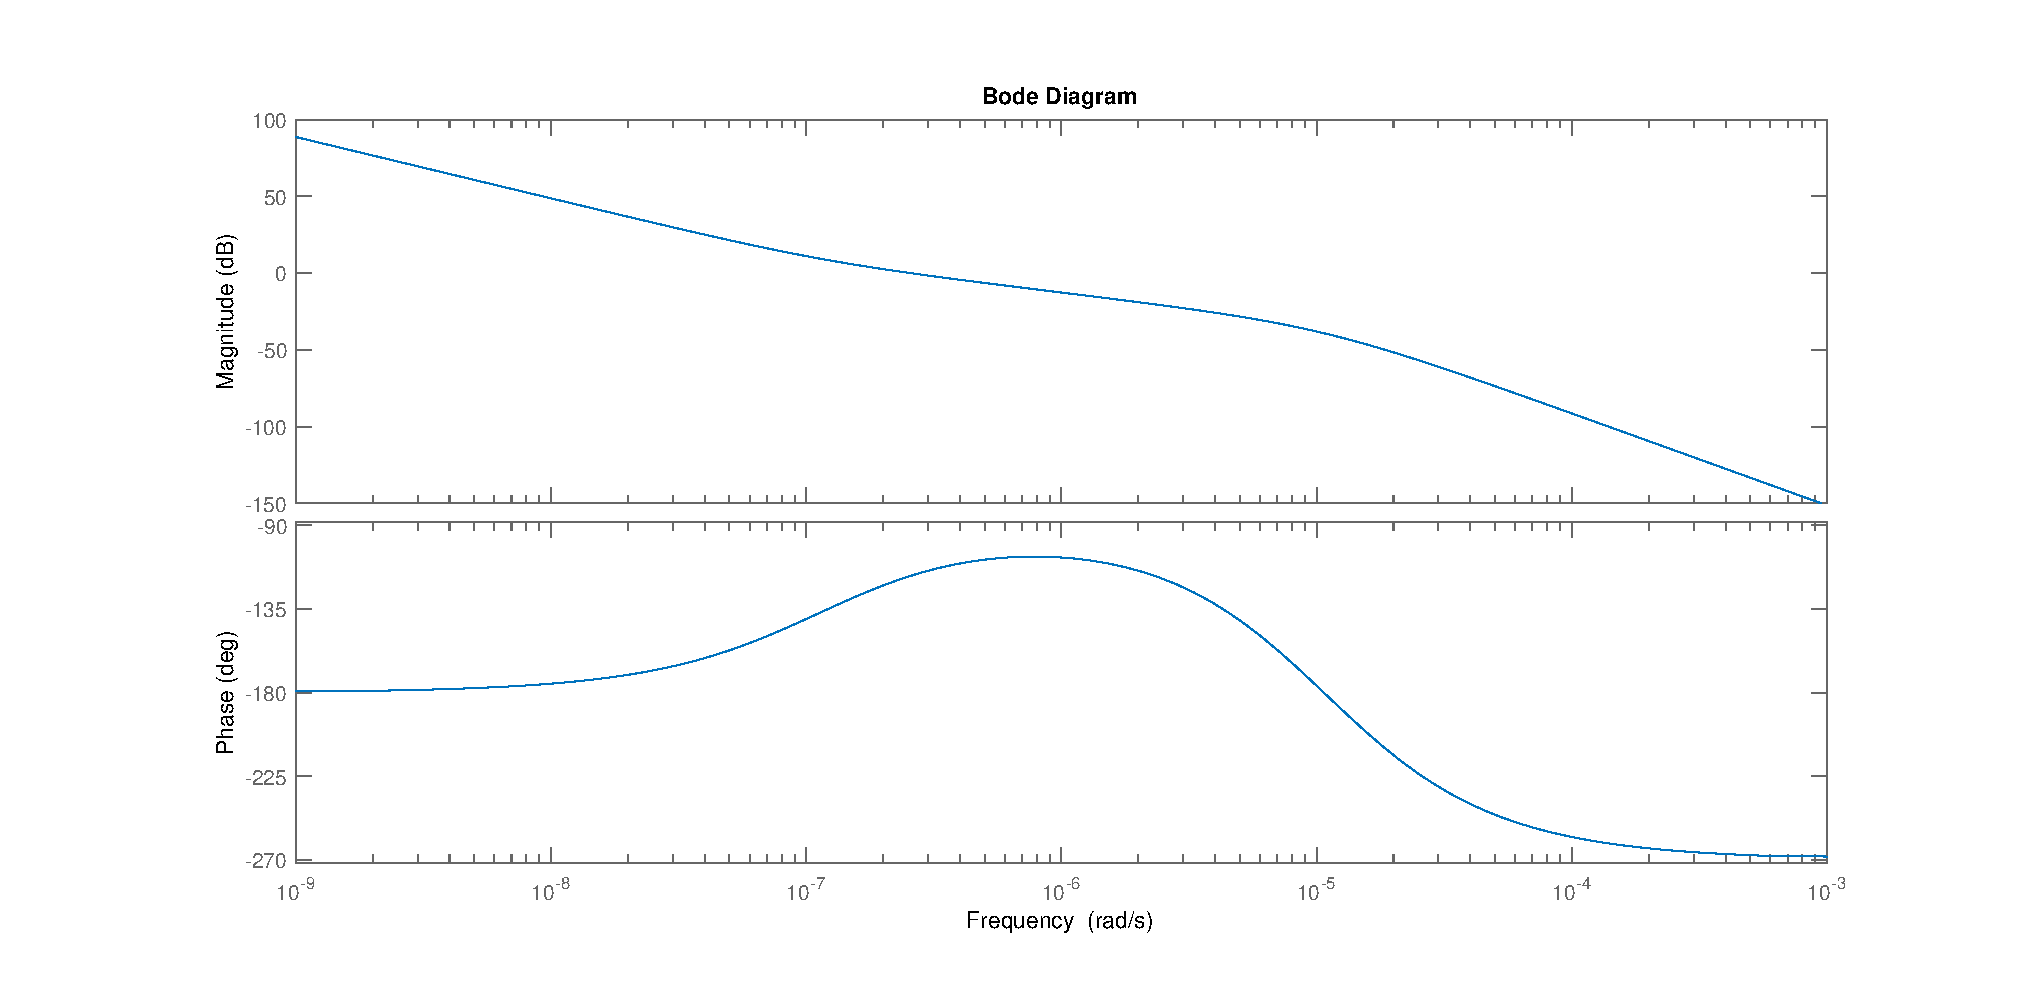
\includegraphics[width=0.9\linewidth]
	{figures/Bode_L.eps}
	\caption{Bode diagram of the loop transfer function}
	\label{fig:Bode_L}
\end{figure}
In the modeling, the control input signal (drag force coefficient) was assumed to be able to change instantaneously but in the real system,variations of the orientation of the satellite take times. Therefore, the phase margin must be big enough to allow a delay in the controller. In the bode diagram, the phase margin can be estimated equal to $62^{circ}$ which is enough to accept a large delay due to the small crossover frequency. \\

\subsubsection{Constellation Formation Control} 
Since the formation consists for more than two satellites a second controller is designed to control n satellites around the Earth. The gain vector K computed above can be used to calculate the difference drag force between two neighbours satellites (called $u_a = u_2 - u_1$, $u_b = u_3 - u_2$, ...). Thus, a system of n-1 equations with n unknown variables is obtained. the last equation is chosen to set the minimum value of $u_1$, $u_2$,... equals to $u_min$. We have now a system of n equations with n unknown variables that can be solved to determine the drag force coefficient $u_i$ for each satellite.
%
\subsection{Stability Analysis}
In order to analyze the stability of the distributed formation controller, once more, the system should be written in state space form as in  \eqref{eq:statespacecomplex}. The states are defined as 
\begin{flalign*}
	s = [\theta; \dot{\theta}]
	\label{stateformation}
\end{flalign*}
where $\theta = [\theta_{12};\theta_{23};\theta_{34};\theta_{45};\theta_{56};\theta_{67};\theta_{78}]$ are the angles between neighbor satellites and $\dot{\theta} $ is the time derivative of the in between angles. So the system matrix will be a 14x14 matrix and for $i<8$ satellites, $\dot{s}_{i} = s_{i+7}$ and so $\dot{s(1)} = s(8)$ and so on. Depenting on the above the $A$ matrix can be written as
%
\begin{flalign}
	{A}
	= 
	\begin{bmatrix}
		0_{7x7}& I_{7x7}& \\
		0_{7x7}& 0_{7x7}
	\end{bmatrix} 
\end{flalign}
%
and B matrix with $C = \frac{3 \omega_0^2 R_0}{m} $ and $u = [u_2-u_1;u_3-u_2;...;u_8-u_7]$ can be written as
\begin{flalign}
	{B}
	= 
	\begin{bmatrix}
		0_{7x1}& \\
		C_{7x1}
	\end{bmatrix}
\end{flalign}
%
The controller gain that has be found in section\ref{46}, $K = [K_{1} K_{2}]$, now can be written as $K_{s} = [K_{1}I_{7x7},  K_{1}I_{7x7}]$ and  by using a control law $u = -Ks$ a stability analysis can be made by using a Lyapunov candidate function as $V = s^{T}s$ where $V>0$, $\forall s\neq0 $. Inserting $K_{s}$ in the state space equation is obtained
%
\begin{flalign}
	&{\dot{s}} ={(A  + BK_{s})s}
	\label{eq:statespacecomplex2}
\end{flalign}  
%
From lyapunov stability criterion it has to be shown that $\dot{V} <0$,$\forall s\neq0 $. The derivative of the candidate function can be written as 
%
\begin{flalign}
	&{\dot{V}} ={\dot{s}^{T}s+s^{T}\dot{s}}
	\label{eq:statespacecomplex3}
\end{flalign}
%
and this is equal to 
%
\begin{flalign}
	&{\dot{V}} ={s^{T}(A-BK)s + s^{T}(A-BK)s}
	\label{eq:statespacecomplex4}
\end{flalign}
%
so the only thing that has to be shown in order for the system to be stable is to show that the eigenvalues of $A-BK<0$. 
%
\section{Simulation and results}
 First the simulation results of the control scheme between two satellites are shown. The reference angle is chosen to be $60^{o}$. The inputs to the controller are $\Delta\theta$ and $\dot{\theta}$, where $\Delta\theta = \theta - \theta{ref}$ and $\dot{\theta} = w_2 - w_1$. In order to smooth the high frequency  oscillations from $\theta$, $w_1$ and $w_2$ to the controller a low pass filter is used. The control design is similar to PD controller. In \figref{fig:distancecontrol} is shown the response of the controller. The gain similar to proportional gives an overshoot with nice rise time and the gain similar to the derivative part gives good settling time with small steady state error.   
%
\begin{figure}[H]
	\centering
	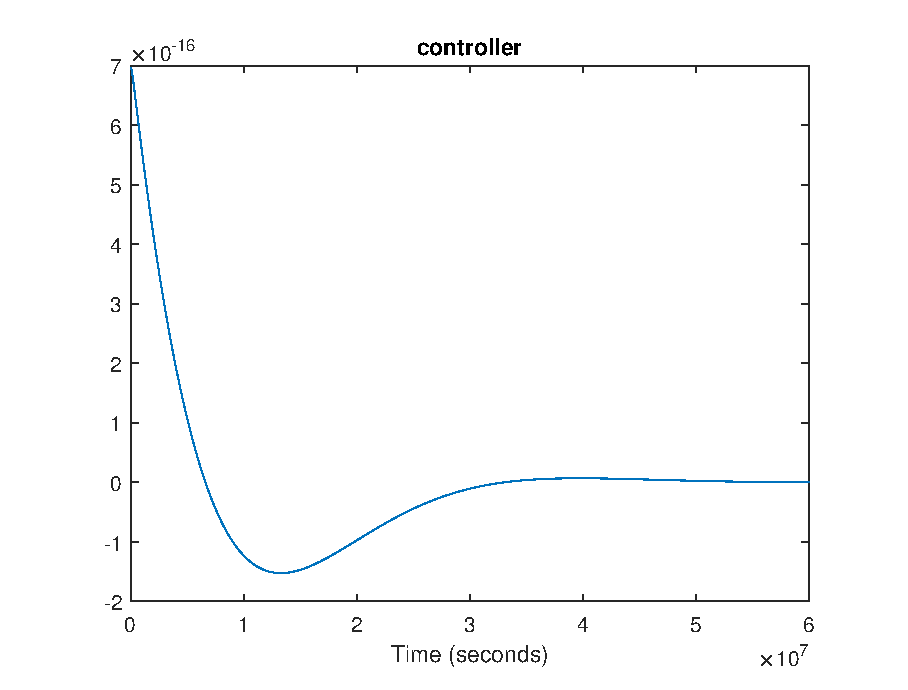
\includegraphics[width=0.9\linewidth]
	{figures/distance_control_twosat.eps}
	\caption{Distance control of two satellites }
	\label{fig:distancecontrol}
\end{figure}
%
The \figref{fig:distancecontrol2} shows that the angle settles at 60 degrees which is the desired angle in between the satellites. Since the satellites are assumed to start at the same position it can be seen that the angle at the beginning is at $0^{o}$. 
%
\begin{figure}[H]
	\centering
	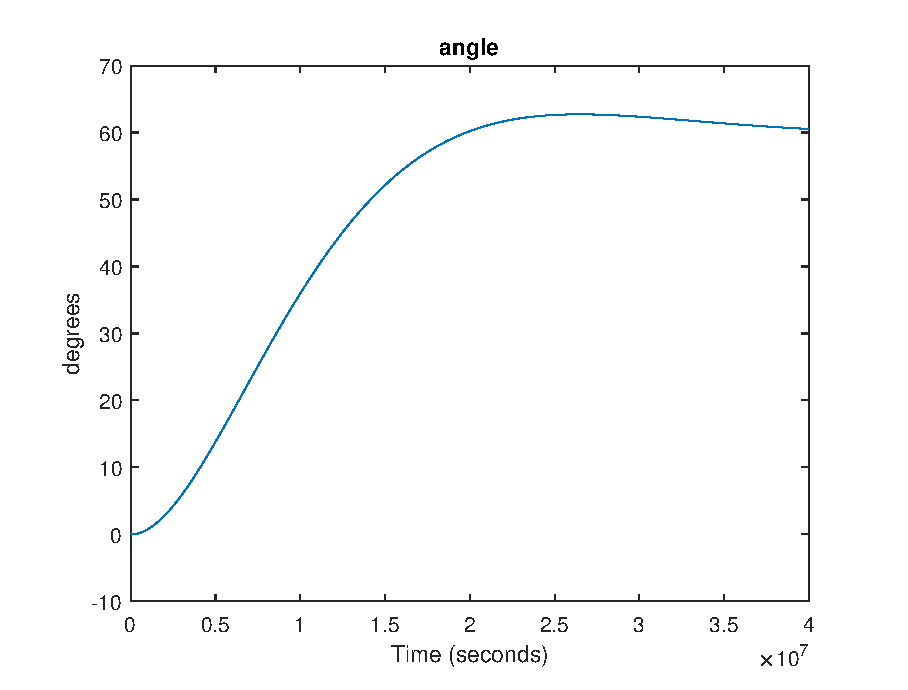
\includegraphics[width=0.9\linewidth]
	{figures/newangle.eps}
	\caption{Angle between two satellites }
	\label{fig:distancecontrol2}
\end{figure}
%
The \figref{fig:distancecontrol3} and \figref{fig:distancecontrol4} are shown the input signal to the satellite 1 and satellite 2 respectively, as a function of the drag force. 
%
\begin{figure}[H]
	\centering
	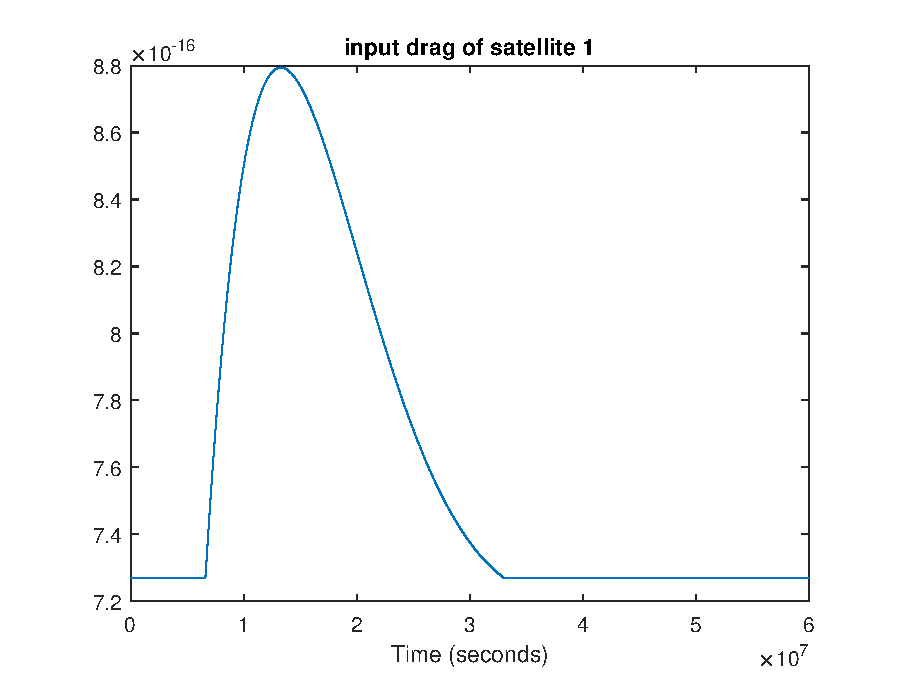
\includegraphics[width=0.9\linewidth]
	{figures/input_drag_sat1.eps}
	\caption{The applied input of satellite 1 as a function of drag force  }
	\label{fig:distancecontrol3}
\end{figure}
%
\begin{figure}[H]
	\centering
	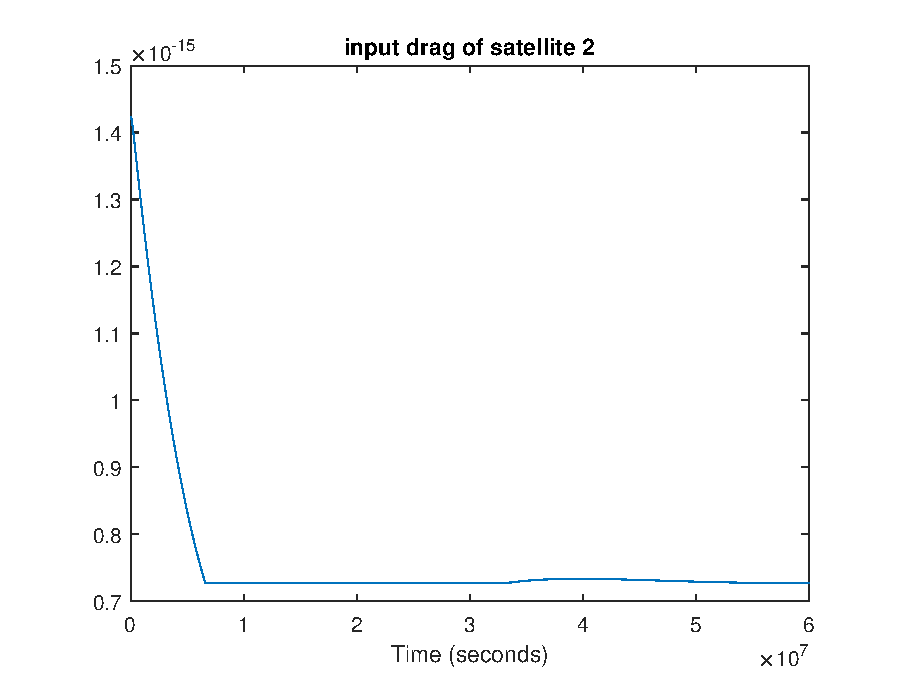
\includegraphics[width=0.9\linewidth]
	{figures/input_drag_sat2.eps}
	\caption{The applied input of satellite 2 as a function of drag force  }
	\label{fig:distancecontrol4}
\end{figure}
%
Since the behavior of the controller and the simulation result for the angle are  good enough between two satellites, the next results to be shown are the results of the simulation between $n$ satellites around the earth. 
%